\chapter{Cuidar la naturaleza}\label{ch:g2:caring-for-nature}

Después de la merienda campestre, una familia deja el prado
exactamente como lo encontró; otra deja bolsas, chapas de botella y un
hormiguero pisoteado. Los conejos, las hormigas y las margaritas del
prado no nos pueden pedir que tengamos cuidado --- pero son \omterm{def:g1:living-or-not:living}{seres
vivos} que comparten nuestros sitios, y cómo nos portamos en la
\omterm{def:g2:caring-for-nature:environment}{naturaleza} les importa. Cuidar la \omterm{def:g2:caring-for-nature:environment}{naturaleza} es algo que cualquiera
puede aprender, a cualquier edad.

\section{La naturaleza es donde viven los seres vivos}

\begin{definition}[La naturaleza y el entorno]\label{def:g2:caring-for-nature:environment}
La \emph{naturaleza}\index{naturaleza} es el mundo de los \omterm{def:g1:living-or-not:living}{seres vivos}
y de lo que los rodea: prados, bosques, charcas, mares --- y el aire,
el agua y la tierra de los que dependen. Aquello que rodea a un \omterm{def:g1:living-or-not:living}{ser
vivo} y de lo que depende se llama su \emph{entorno}\index{entorno}.
\end{definition}

\begin{example}[Todo es la casa de alguien]\label{ex:g2:caring-for-nature:home}
Un tronco podrido del bosque parece basura --- y es un palacio:
escarabajos bajo la corteza, cochinillas debajo, musgo encima, un
erizo pasando el invierno en el hueco. Deshazlo a patadas por
diversión y cuatro familias se quedan sin casa. En la \omterm{def:g2:caring-for-nature:environment}{naturaleza} casi
todo es la casa, la comida o el refugio de alguien.
\end{example}

\begin{omfigure}
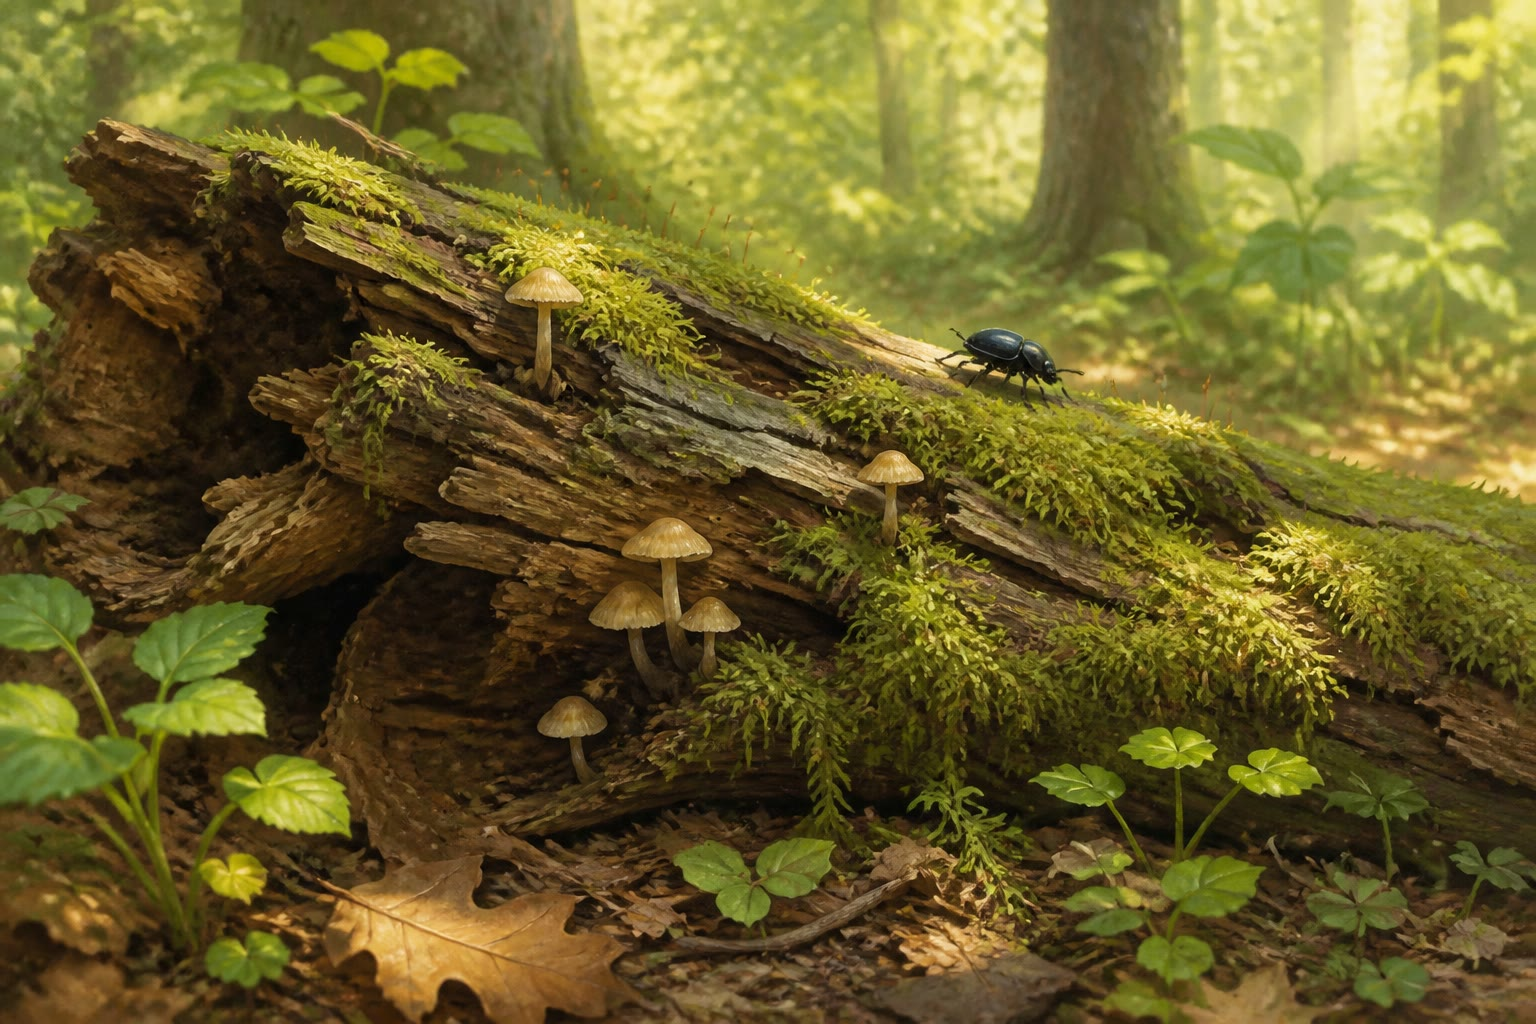
\includegraphics[width=0.62\linewidth]{images/book1/ai/g2-nature-log.jpg}

{\small El tronco podrido que en realidad es un palacio: musgo en el
tejado, setas en las paredes, un escarabajo en el pasillo.}
\end{omfigure}

\begin{remark}[Nosotros formamos parte]\label{rem:g2:caring-for-nature:part}
Las personas también somos \omterm{def:g1:living-or-not:living}{seres vivos}: el aire que respiramos, el
agua que bebemos y la comida que comemos vienen todos de la
\omterm{def:g2:caring-for-nature:environment}{naturaleza}. Cuidarla no es solo ser buenos con los conejos --- es
cuidar el mundo del que vivimos nosotros mismos, como decía el
\cref{ch:g2:where-animals-live} de todos los \omterm{def:g2:where-animals-live:habitat}{hábitats}.
\end{remark}

\section{Qué hace daño y qué ayuda}

\begin{proposition}[Gestos pequeños, daño de verdad]\label{prop:g2:caring-for-nature:harm}
En la \omterm{def:g2:caring-for-nature:environment}{naturaleza}, el daño casi nunca viene de querer portarse mal ---
viene de no pensar:
\begin{itemize}
  \item la basura se queda años y puede atrapar o envenenar \omterm{def:g1:animals-around-us:animal}{animales};
  \item coger todas las \omterm{def:g1:plants-around-us:parts}{flores} no deja ninguna para hacer \omterm{def:g2:from-seed-to-plant:seed}{semillas} ---
        ni ninguna para las abejas;
  \item los gritos y las persecuciones espantan a los \omterm{def:g1:animals-around-us:animal}{animales} lejos de
        su comida y de sus crías;
  \item las orillas pisoteadas, las piedras dadas la vuelta y las \omterm{def:g1:plants-around-us:tree}{ramas}
        rotas deshacen cada una una casita.
\end{itemize}
\end{proposition}
\admitted

\begin{example}[La chapa de la botella]\label{ex:g2:caring-for-nature:cap}
Una chapa de plástico que se cae no es nada para nosotros y se queda
en el prado muchísimos años --- los bastantes para que las personas
mayores tengan hijos que se encuentren esa misma chapa. La \omterm{def:g2:caring-for-nature:environment}{naturaleza}
no tiene camión de la basura: lo que dejamos, se queda.
\end{example}

\begin{method}[Las reglas del visitante]\label{met:g2:caring-for-nature:rules}
En plena \omterm{def:g2:caring-for-nature:environment}{naturaleza}:
\begin{enumerate}
  \item llévate a casa toda tu basura --- toda;
  \item mira las \omterm{def:g1:plants-around-us:parts}{flores}, los insectos y los nidos en vez de
        coleccionarlos; coge como mucho unas pocas \omterm{def:g1:plants-around-us:parts}{flores} comunes,
        nunca todas las de una mata;
  \item vuelve a colocar cada piedra y cada tronco que des la vuelta
        --- debajo vive alguien;
  \item no te salgas de los caminos cerca de los sitios frágiles, como
        las orillas de los arroyos;
  \item observa a los \omterm{def:g1:animals-around-us:animal}{animales} de lejos y en silencio, y no toques a
        sus crías.
\end{enumerate}
Deja el sitio de manera que nadie note que estuviste allí.
\end{method}

\begin{example}[Ayudar a propósito]\label{ex:g2:caring-for-nature:help}
Cuidar puede ir más allá de no hacer daño. Un platito de agua en una
ola de calor, un rincón salvaje del jardín sin segar, \omterm{def:g2:from-seed-to-plant:seed}{semillas} para
los pájaros cuando hace frío, una charca de colegio como la del
\cref{ex:g2:where-animals-live:schoolpond}: cada uno de ellos les da a
algunos \omterm{def:g1:living-or-not:living}{seres vivos} comida, agua o una casa que habían perdido.
\end{example}

\section{Separar y ahorrar}

\begin{proposition}[Los residuos se pueden devolver]\label{prop:g2:caring-for-nature:recycle}
Mucho de lo que tiramos se puede volver a usar.
\emph{Separar}\index{separación de residuos} los residuos --- el
vidrio con el vidrio, el papel con el papel, las peladuras al compost
--- permite que las botellas se conviertan en botellas nuevas y que
las peladuras se conviertan en tierra, en vez de que todo se amontone.
Y lo que se \emph{ahorra} --- agua, papel, electricidad --- no llega
nunca a ser un residuo.
\end{proposition}
\admitted

\begin{example}[El cubo de compost]\label{ex:g2:caring-for-nature:compost}
Los corazones de manzana y las peladuras de zanahoria, en un cubo de
compost, se convierten despacio en tierra oscura y desmenuzada --- con
la ayuda de lombrices, cochinillas y \omterm{def:g1:living-or-not:living}{seres vivos} demasiado pequeños
para verlos. La primavera siguiente, esa tierra alimenta los tomates.
No se desperdició nada; las peladuras volvieron al ciclo de la vida.
\end{example}

\begin{remark}[Las manos pequeñas cuentan]\label{rem:g2:caring-for-nature:count}
Cerrar el grifo mientras te lavas los dientes, usar las dos caras del
papel, el cubo de compost, la basura que te llevas a casa: cada cosa
es pequeña, y millones de personas las hacen --- o no. La \omterm{def:g2:caring-for-nature:environment}{naturaleza}
se cuida, o se estropea, sobre todo en elecciones diarias pequeñas
como las tuyas.
\end{remark}

\section{Ejercicios}

\begin{exercise}[$\star$]\label{exo:g2:caring-for-nature:1}
¿Qué es el \omterm{def:g2:caring-for-nature:environment}{entorno} de un \omterm{def:g1:living-or-not:living}{ser vivo}? Nombra tres cosas del tuyo que
vengan de la \omterm{def:g2:caring-for-nature:environment}{naturaleza}.
\end{exercise}

\begin{exercise}[$\star$]\label{exo:g2:caring-for-nature:2}
¿Quién se puede quedar sin casa cuando se deshace a patadas un tronco
podrido? Nombra tres habitantes del \cref{ex:g2:caring-for-nature:home}.
\end{exercise}

\begin{exercise}[$\star$]\label{exo:g2:caring-for-nature:3}
Da cuatro reglas del visitante del \cref{met:g2:caring-for-nature:rules}.
\end{exercise}

\begin{exercise}[$\star$]\label{exo:g2:caring-for-nature:4}
¿Por qué tiene que irse la basura a casa con nosotros? Responde con la
chapa de botella del \cref{ex:g2:caring-for-nature:cap}.
\end{exercise}

\begin{exercise}[$\star$]\label{exo:g2:caring-for-nature:5}
¿Por qué no hay que coger todas las \omterm{def:g1:plants-around-us:parts}{flores} de una mata? Da las dos
razones de la \cref{prop:g2:caring-for-nature:harm}.
\end{exercise}

\begin{exercise}[$\star$]\label{exo:g2:caring-for-nature:6}
¿Qué les pasa a los corazones de manzana en un cubo de compost? ¿Quién
hace el trabajo y qué obtenemos al final?
\end{exercise}

\begin{exercise}[$\star$]\label{exo:g2:caring-for-nature:7}
Di dos maneras de ayudar a la \omterm{def:g2:caring-for-nature:environment}{naturaleza} a propósito, sacadas del
\cref{ex:g2:caring-for-nature:help}.
\end{exercise}

\begin{exercise}[$\star$]\label{exo:g2:caring-for-nature:8}
Pruébalo: en tu próximo paseo, cuenta los trozos de basura que veas
(sin tocar los peligrosos). ¿Qué clase es la más frecuente? ¿Adónde
debería haber ido cada una?
\end{exercise}

\begin{exercise}[$\star\star$]\label{exo:g2:caring-for-nature:9}
En la charca, Emma quiere llevarse tres \omterm{ex:g2:animals-grow-up:frog}{renacuajos} a casa en un bote
``para que crezcan seguros''. Con este capítulo y el
\cref{exo:g2:where-animals-live:10}, ¿qué le aconsejarías en su lugar?
\end{exercise}

\begin{exercise}[$\star\star$]\label{exo:g2:caring-for-nature:10}
``Una chapa de botella no es nada''. Usa la
\cref{rem:g2:caring-for-nature:count} para responder: ¿qué pasa cuando
un millón de visitantes piensa cada uno la misma frase --- en la mala
dirección y en la buena?
\end{exercise}
